\section{Differenzation}
Die partielle Ableitung gbt a n welche Steigung die Funktion $f$ in die Richtung hat, nach welcher sie abgeleitet wurde. Höhere Ableitungen können durch mehrfach Ableitung erhalten werden. Dabei darf die Reihenfolge der einzelnen partiellen Differzationen beliebig vertauscht werden $f_{xy} = f_{yx}$, wenn die partiellen Ableitung $n$-ter Ordnung stetig sind.


Das \textbf{Differential}\label{differential} ist $dy = f_x(x;y)dx + f_y(x;y)dy$ und kann mit
\[
\underbrace{f(x;y) - f(x_0;y_0)}_\text{dy} = f_x(x_0; y_0)\underbrace{(x - x_0)}_\text{dx} + f_y(x_0;y_0)\underbrace{(y - y_0)}_\text{dy}
\] berechnet werden

\subsection{Linearisation}
Um eine Hyper-Ebene der Funktion $f$ zu erstellen, benötigt man die \textbf{Jacobian Matrix} $\mathbf{J}_f$ einer Funktion $f$.
\[
\mathbf{J}_{\vec{f}}(\vec{x}_0) = \frac{d}{dx}\vec{f}(x) = \nabla\vec{f} = \begin{pmatrix}
	\frac{\partial f_1}{dx_1} & \dots & \frac{\partial f_1}{dx_n} \\
	\vdots & \ddots & \vdots \\
	\frac{\partial f_m}{dx_1} & \dots & \frac{\partial f_m}{dx_n} \\
\end{pmatrix} \qquad \in \mathbb{R}^{m \times n}
\]
Die Liniarisation kann nun implizit
\[
g(\vec{x}) \approx \vec{f}(\vec{x_0}) + \mathbf{J}_{\vec{f}}(\vec{x}_0) \cdot (\vec{x} - \vec{x}_0)  \qquad \vec{x} \approx \vec{x}_0
\]
oder explizit gefunden werden:
\begin{align*}
	g(x_0; \dots; x_m) \approxeq& f(x_0^{(0)}; \dots; x_m^{(0)}) + f_{x_0}(x_0^{(0)}; \dots; x_m^{(0)})(x_1-x_1^{(0)}) +\\ 
	&\dots + f_{x_m}(x_0^{(0)}; \dots; x_m^{(0)})(x_m-x_m^{(0)})
\end{align*}

\subsection{Steigung}
Um eine implizite Steigung $m$ einer Kurve zu berechnen. Siehe auch \ref{gradient}.
\[
m = - \frac{f_x(x_0;y_0)}{f_y(x_0; y_0)}
\]

\noindent Um eine \textbf{Richtungsableitung} $\vec{r}$ zu erhalten, kann 
\[
\frac{\partial f}{\partial \vec{r}} = f_x(x_0;y_0)\cos(\alpha) + f_y(x_0;y_0)\sin(\alpha)
\]


\subsection{Fehlerfortpflanzung}
Das Messergebnis zweier gemessener Grössen $x$ und $y$ liegen in der Form $x = \overline{x} \pm \sigma_{\overline{x}}$ und $y = \overline{y} \pm \sigma_{\overline{y}}$ vor. Diese werden in der Form $z$ dargestellt:
\[
z = \overline{z} \pm \sigma_{\overline{z}} \approx f(\overline{x}; \overline{y}) \pm \sqrt{[f_x(\overline{x}, \overline{y})\cdot\sigma_{\overline{x}}]^2 + [f_y(\overline{x}, \overline{y})\cdot\sigma_{\overline{y}}]^2}
\]
Die Standardabweichung $\sigma$ kann durch 
\[
\sigma_{\overline{z}} = \frac{1}{\sqrt{n}}\cdot\sigma_z = \frac{1}{\sqrt{n}}\cdot\sqrt{\frac{\sum\limits_{i=1}^{n}(z_i - \overline{z})^2}{n-1}}
\]
berechnet werden.

\subsection{Gradient}\label{gradient}
Der Gradient ist ein Vektor, der alle ersten Partiellen Ableitungen der Funktion $f$ enthält:
\[
\nabla f(x_1,\dots,x_n) = \begin{pmatrix}
	\frac{\partial f}{\partial x_1} = f_{x_1}(\dots) \\
	\dots \\
	\frac{\partial f}{\partial x_n} = f_{x_n}(\dots)
\end{pmatrix}
\]
\textbf{Eigenschaften}\\
\begin{itemize}[nosep]
	\item Gradient zeigt in Richtung des grössten Anstiegs
	\item Die Steigung in diese Richtung beträgt $\left|\nabla f\right|$
	\item Gradient steht senkrecht auf der Niveaulinie
\end{itemize}~\\

\noindent Es kann eine Beliebige Steigung $s$ in Richtung $\vec{r}$ berechnet werden, indem das Skalarprodukt mit den Gradienten berechnet wird:
\[
s = \frac{\partial f(\vec{x})}{\partial \vec{r}} = \nabla f(\vec{x}) \circ \vec{r} \qquad |\vec{r}| = 1
\]
\noindent Achtung: Richtung muss immer ein Einheitsvektor sein: $\vec{r} = \frac{\vec{r}_0}{\left|\vec{r}_0\right|}$

\subsection{Extrema von Funktionen}
An Extremalstellen ist der grösste Anstieg gleich $0$.
\[\nabla f = \vec{0}\]

\noindent\begin{minipage}{\columnwidth}
	\begin{minipage}{0.7\textwidth}
		Es kommen für Extrema folgende Punkte im Definitionsbereich $\mathbb{D}_f$ in Frage:
		\begin{enumerate}[nosep]
			\item Randpunkte von $\mathbb{D}_f$
			\item Punkte, in denen $\nabla f$ nicht existiert
			\item Punkte, in denen $\nabla f = \vec{0}$
		\end{enumerate}
	\end{minipage}%%% to prevent a space
	\begin{minipage}{0.3\textwidth}
		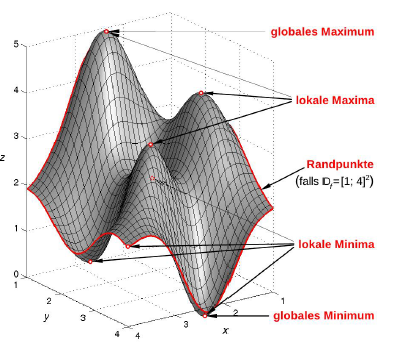
\includegraphics[width=\columnwidth]{Images/extrema}
	\end{minipage}
\end{minipage}

Für das bestimmen des Punktes kann die Hesse-Matrix benutzt werden. Dazu alle Extremalstellen Kandidaten in die Hesse-Matrix einfügen und Definitheit bestimmen zB mit Eigenwerten ($\det(\mathbf{H} - \textcolor{red}{\lambda} E) = 0$), Diagonalmatrix, Hurwitz-Kriterium, Chorlesky-Zerlegung oder Quadratische-Ergänzung. Die Definitheit der Hesse-Matrix sagt Type der Extremalstelle aus.
\[
\mathbf{H}_f(\vec{x}) = \begin{pmatrix}
	\frac{\partial^2 f}{\partial x_1 \partial x_1}(\vec{x}) & \dots & \frac{\partial^2 f}{\partial x_1 \partial x_n}(\vec{x})\\
	\vdots & \ddots & \vdots \\
	\frac{\partial^2 f}{\partial x_n \partial x_1}(\vec{x}) & \dots & \frac{\partial^2 f}{\partial x_n \partial x_n}(\vec{x})
\end{pmatrix}
\]

\noindent\textbf{Tip:} Hat die $\mathbf{H}_f(\vec{x}))$ auf der Hauptdiagonale Werte $>0$ \underline{und} $<0$ oder \underline{nur} $=0$, dann ist der Punkt sicher ein Sattelpunkt.\\~\\

\begin{align*}
	\mathbf{H}_f(\vec{x}) = \begin{cases*}
		\forall \lambda_i < 0, & \text{Lokales Maximum, Neg definit} \\
		\forall \lambda_i > 0, & \text{Lokales Minimum, Pos definit} \\
		\lambda_i < 0 \cup \lambda_i > 0 & \text{Sattelpunkt, indefinit} \\
		\lambda_i = 0 & \text{Weitere Untersuchungen, semidefinit}
	\end{cases*}
\end{align*}

\noindent\textbf{Tip:} Für 2D Funktionen kann $\Delta = f_{xx}f_{yy} - f^2_{xy}$ berechnet werden. Für $\Delta>0$ und $f_{xx}(\vec{x})<0$ lokales Maximum oder $f_{xx}(\vec{x})>0$ lokales Minimum. Bei $\Delta < 0$ Sattelpunkt und $\Delta = 0$ keine Aussage. 

\subsubsection{Nebenbedingungen}
Bestimmt alle Extremalpunkte mit $m$ Anzahl Nebenbedingunge $g_m$ für Funktion $f$. Mögliche Extremalpunkte im Definitionsbereich $\mathbb{D}_f$ sind:
\begin{itemize}[nosep]
	\item Randpunkte von $f$ welche $g_m$ erfüllen
	\item Punkte, in denen $\nabla f$ nicht existiert oder linearabhängig sind und Nebenbedingungen $g_m$ erfüllen
\end{itemize}
Alle oberen und folgenden Punkte sind mögliche Extra, welche wiedrum mit der Hessian-Matrix bestimmt werden können.
\begin{enumerate}[nosep]
	\item Nebenbedingungen nach $0$ umstellen
	\item Lagrange $\mathcal{L}$ Funktion bestimmen $\Rightarrow \mathcal{L}(\vec{x};\vec{\lambda}) = f(\vec{x}) + \sum_{i=1}^{m}\lambda_i\cdot g_i(\vec{x})$
	\item Gleichung $\nabla\mathcal{L} \eqi 0$ lösen. Immer mit Additionsverfahren alle $\lambda_i$ entfernen! Anschliessend LGS lösen.
\end{enumerate}

\noindent\textbf{Hinweis} für 2 Variablen\\
Für 2 Dimensionale Extremalaufgaben mit Funktion $f$ und Nebenbedingung $g$ folgende Vereinfachung:
\begin{enumerate}[nosep]
		\item Nebenbedingungen nach $0$ umstellen
	\item Randpunkte von $\mathbb{D}_f$, falls sie die Nebenbedingung erfüllen
	\item Punkte, in denen der $\nabla f$ und/oder $\nabla g$ nicht existieren aber die Nebenbedingungen $g = 0$ erfüllen
	\item Lösungen des LGS $\begin{vmatrix}
		f_x \cdot g_y = f_y \cdot g_x \\
		g = 0
	\end{vmatrix}$
\end{enumerate}


